% Author: Izaak Neutelings (June 2020)
% Inspiration:
%   https://www.researchgate.net/figure/a-Refractive-index-and-b-dispersion-of-bulky-soft-glasses-NC21-LLF1-SF6-and-F2-As_fig1_236110630
%   https://link.springer.com/article/10.1007/s11082-014-9979-y
\documentclass[border=3pt,tikz]{standalone}
\usepackage{siunitx}
\usetikzlibrary{calc}
\usetikzlibrary{intersections}
\usetikzlibrary{fadings}
\tikzset{>=latex} % for LaTeX arrow head

\colorlet{myblue}{blue!80!black}
\colorlet{myred}{black!50!red}
\colorlet{glasscol}{blue!10}
\tikzstyle{glass}=[top color=glasscol!90!black,bottom color=glasscol!90!black,middle color=glasscol,shading angle=40]


\begin{document}


%% PRISM + REFRACTION
%\begin{tikzpicture}
%  \def\N{6}
%  \def\L{2.8}
%  \def\na{1.0} % air
%  \def\angi{50}
%  \coordinate (O) at (0,0);
%  \coordinate (R) at (\L,0);
%  \coordinate (T) at (60:\L);
%  \coordinate (I) at (60:0.5*\L);
%  
%  % MEDIUM
%  \draw[line width=0.8,blue]  (I)++(150+\angi:0.3*\L) -- (I) --++ (\angi-30:0.007*\L);
%  \draw[line width=0.6,white] (I)++(150+\angi:0.3*\L) -- (I) --++ (\angi-30:0.007*\L);
%  \fill[glass] (O) -- (T) -- (R) -- cycle;
%  \path[name path=side] (T) -- (R);
%  
%  % LIGHT BEAMS
%  % https://tex.stackexchange.com/questions/230227/creating-a-rainbow-color-macro
%  \foreach \i [evaluate={
%      \ng=1.6-\i*0.2/\N;
%      \lamb=410+\i*320/\N;
%      %\len=1.5+\i*0.8/\N;
%      \angr=asin(\na/\ng*sin(\angi));
%      \angR=asin(\ng/\na*sin(60-\angr));
%      \dang=-30+\i*60/\N;}] in {0,...,\N}{
%    \definecolor{tmpcol}{wave}{\lamb}
%    \colorlet{mycol}[rgb]{tmpcol}
%    \path[name path=beam1] (I) --++ (-30+\angr:0.8*\L);
%    \draw[mycol,name intersections={of=side and beam1,name=f}] %wave={\len}
%      (I)++(\dang:0.0028*\L) -- (f-1) --++ (30-\angR:0.4*\L); %node[scale=0.3] {\angR};
%  }
%  %\foreach \i in {1,2}{
%  %  \draw[line width=0.59,white,path fading=east] (I)++(20:0.002*\L) --++ (1:0.08*\L);
%  %  \draw[line width=0.59,white,path fading=east] (I)++(20:0.002*\L) --++ (1:0.03*\L);
%  %}
%  \coordinate (IT) at ($(I)+(60:0.006*\L)$);
%  \fill[white,path fading=east]
%    (IT) --++ (-120:0.012*\L) --++ (-1.3:0.10*\L) --++ (80:0.018*\L) -- cycle;
%  \fill[white,path fading=east]
%    (IT) --++ (-120:0.012*\L) --++ (-1.3:0.06*\L) --++ (80:0.0148*\L) -- cycle;
%  
%\end{tikzpicture}


% PRISM + REFRACTION
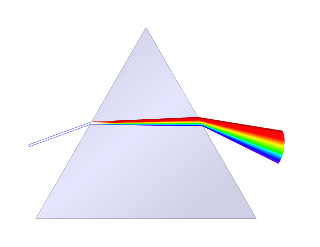
\begin{tikzpicture}
  \def\N{200} % number of rainbow rays
  \def\L{2.8}
  \def\na{1.0} % air
  \def\angi{50}
  \coordinate (O) at (0,0);
  \coordinate (R) at (\L,0);
  \coordinate (T) at (60:\L);
  \coordinate (I) at (60:0.5*\L);
  
  % MEDIUM
  \draw[line width=0.8,blue]  (I)++(150+\angi:0.3*\L) -- (I) --++ (\angi-30:0.01*\L);
  \draw[line width=0.6,white] (I)++(150+\angi:0.3*\L) -- (I) --++ (\angi-30:0.01*\L);
  \fill[glass] (O) -- (T) -- (R) -- cycle;
  \path[name path=side] (T) -- (R);
  
  % LIGHT BEAMS
  % https://tex.stackexchange.com/questions/230227/creating-a-rainbow-color-macro
  \begin{scope}
    \coordinate (IT) at ($(I)+(60:0.006*\L)$);
    \clip (O) -- (T) -- (1.08*\L,0.45*\L) to[out=-35,in=20,looseness=1]
          (1.04*\L,0.2*\L) -- (R) -- cycle;
    \foreach \i [evaluate={
        \f=\i/\N;
        \ng=1.6-\f*0.2;
        \lamb=410+\f*320;
        \angr=asin(\na/\ng*sin(\angi));
        \angR=asin(\ng/\na*sin(60-\angr));
        \dl=0.0108*(1-\f)*\L;}] in {0,...,\N}{
      \definecolor{tmpcol}{wave}{\lamb}
      \colorlet{mycol}[rgb]{tmpcol}
      \path[name path=beam1] (I) --++ (-30.1+\angr:0.8*\L);
      \path[name path=beam2] (I) --++ (-30.0+\angr:0.8*\L);
      \coordinate (IT2) at ($(I)+(57:0.005*\L)+(-120:\dl)$);
      \fill[mycol,name intersections={of=side and beam1,name=t},
            name intersections={of=side and beam2,name=b}] %wave={\len}
        (IT2) -- (t-1) -- ($(t-1)+(30.0-\angR:0.4*\L)$)
        -- ($(b-1)+(30.1-\angR:0.4*\L)$) -- (b-1) -- ($(IT2)+(-120:-0.001*\L)$); %node[scale=0.3] {\angR};
    }
  \end{scope}
  \fill[white,path fading=east]
    (IT) --++ (-120:0.012*\L) --++ (-1.3:0.06*\L) --++ (80:0.015*\L) -- cycle;
  \fill[white,path fading=east]
    (IT) --++ (-120:0.012*\L) --++ (-1.3:0.10*\L) --++ (80:0.018*\L) -- cycle;
  
\end{tikzpicture}


% REFRACTION
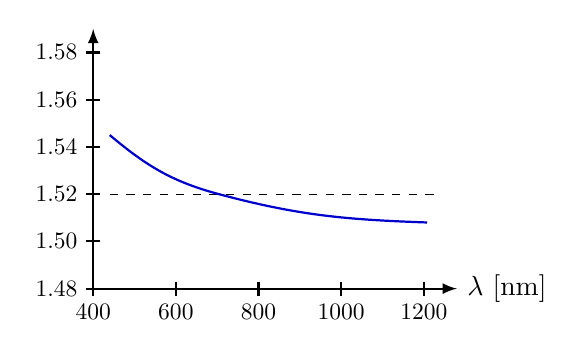
\begin{tikzpicture}
  \def\Nx{4}
  \def\Ny{5}
  \def\xmax{4.2}
  \def\ymax{3}
  \def\nave{0.4*\ymax}
  \coordinate (L) at (0.05*\xmax,0.65*\ymax);
  \coordinate (M) at (0.38*\xmax,0.40*\ymax);
  \coordinate (R) at (1.01*\xmax,0.28*\ymax);
  \def\tick#1#2{\draw[thick] (#1) ++ (#2:0.03*\ymax) --++ (#2-180:0.06*\ymax)}
  
  % AXES
  \draw[->,thick] (0,0) -- (1.1*\xmax,0) node[right] {$\lambda$ [\si{nm}]};
  \draw[->,thick] (0,0) -- (0,1.1*\ymax);
  \foreach \i [evaluate={\x=\i*\xmax/\Nx;\lamd=int(400+\i*200)}] in {0,...,\Nx}{
    \tick{\x,0}{90} node[below,scale=0.85] {$\lamd$};
  }
  \pgfkeys{/pgf/number format/precision=2} % decimal precision
  \foreach \i [evaluate={\y=\i*\ymax/\Ny;}] in {0,...,\Ny}{
    \pgfmathparse{1.48+\i*0.02}
    \pgfmathroundtozerofill{\pgfmathresult}
    \pgfmathsetmacro\n{\pgfmathresult}
    \tick{0,\y}{0} node[left,scale=0.85] {$\n$};
  }
  
  % LINE
  \draw[dashed] (0.05*\xmax,\nave) -- (1.05*\xmax,\nave);
  \draw[myblue,thick]
    (L) to[out=-40,in=165,looseness=1] (M)
        to[out=-15,in=178,looseness=1] (R);
  
\end{tikzpicture}



\end{document}